\documentclass[journal]{IEEEtran}

% Working IEEEtran journal manuscript for the JBHI ECG study.
% Template reference:
% templates/ieee-jbhi/IEEEtran/IEEEtran/bare_jrnl.tex

\usepackage{cite}
\usepackage{amsmath,amssymb}
\usepackage{booktabs}
\usepackage{graphicx}
\usepackage{url}

\graphicspath{{overleaf_jbhi_submission/figures/}}

\begin{document}

\title{Empirical Privacy-Risk Analysis of ECG Representations:
Same-Record Linkability, Attribute Inference, and Waveform Reconstruction}

\author{Tiago Patrício, Luís Nunes, and Carlos Serrão%
\thanks{This work was partially supported by national funds through
Funda\c{c}\~ao para a Ci\^encia e a Tecnologia, I.P. (FCT), ISTAR-Iscte
Pluriannual Projects UID/04466/2025
(\protect\url{https://doi.org/10.54499/UID/04466/2025}).}%
\thanks{All authors are with ISTA -- School of Technology and Architecture,
ISCTE -- University Institute of Lisbon, Lisbon, Portugal.
Corresponding author: Tiago Patrício (e-mail: tjpoa@iscte-iul.pt).}}

\maketitle

\begin{abstract}
Compact electrocardiogram representations may retain record-specific structure
after direct identifiers are removed. This study evaluates their utility,
same-record linkability, linkage-mediated attribute inference, and waveform
reconstruction under one matched protocol. We filtered 45,151 12-lead,
10-second PhysioNet recordings, divided each into nine overlapping two-second
segments, and extracted 208 handcrafted features. A three-seed comparison
examined the handcrafted features, two 8-dimensional linear projections, an
8-dimensional utility-supervised encoder, and two Gaussian-perturbed encoder
variants. Handcrafted features achieved segment and record balanced accuracies
of 0.832 and 0.860, with pairwise linkability of 0.999 measured by the area
under the receiver operating characteristic curve. The encoder achieved 0.865,
0.898, and 0.882, respectively. Gaussian perturbation achieved 0.839, 0.894,
and 0.807. In a gallery with one true match among 1,000 candidates, top-ranked
retrieval fell from 0.887 with handcrafted features to 0.084 with the encoder
and 0.014 after perturbation. Attacker-selected grouping added little to sex
and age inference. Reconstruction from handcrafted features produced a percent
root-mean-square difference of 96.5\%, and neither oracle nor attacker-selected
averaging improved anchor reconstruction. Reduced dimension and weak
reconstruction did not imply unlinkability. The findings are limited to the
stated same-record protocol and do not establish cross-session re-identification
resistance or end-to-end differential privacy. For biomedical data sharing,
compact electrocardiogram representations should be evaluated for linkability
before release.
\end{abstract}

\begin{IEEEkeywords}
electrocardiography, health data privacy, linkability, waveform reconstruction,
representation learning
\end{IEEEkeywords}

\section{Introduction}
\label{sec:introduction}

Electrocardiogram (ECG) recordings support rhythm analysis, diagnosis, risk
stratification, and the development of data-driven clinical tools. Their value
for secondary use is accompanied by a privacy concern: physiological
morphology, timing, amplitude, and inter-lead structure may preserve stable
record-specific information even when direct identifiers are removed. ECG has
also been investigated as a biometric signal, making it important to
distinguish clinical utility from the possibility of linkage or recognition
\cite{Odinaka2012ECGBiometric,Pereira2023ECGBiometricReview}.

Most privacy evaluations focus on raw signals, model training, or formal
mechanisms. A complementary question is what happens when ECG data are shared
as derived feature vectors or learned embeddings. For example, a data holder
might publish independently generated segment representations without record
identifiers so that downstream users can build rhythm classifiers. An
attacker who can group segments from the same recording can then aggregate
evidence for sensitive attributes. Independently of that grouping success, an
attacker can attempt to invert each released segment representation toward its
source waveform. A representation can reduce dimensionality without preventing this grouping,
or preserve task-relevant information while discarding part of the
record-specific structure. This motivates evaluating utility and linkability
on the same released object.

Prior ECG privacy work commonly studies biometric identification or evaluates
a particular anonymisation mechanism under method-specific release objects and
attacker protocols
\cite{Macierzanka2025SiameseECG,Wang2025ECGLinkage,NolinLapalme2023PrivECG,Lee2026PrivacyECG,Shishir2026PPVAE}.
These studies establish both the threat and the value of defences, but their
heterogeneous designs do not isolate how alternative compact representations
change utility and multiple privacy risks under matched conditions. Rather
than proposing another anonymisation mechanism, this study treats compact ECG
representations as released data products and evaluates them within one
controlled, multi-axis protocol.

This paper asks: \emph{How well do different ECG representations preserve
utility for a record-derived atrial-arrhythmia classification task while
reducing linkability, and what additional attribute-inference or reconstruction
risks remain?} The contributions are:

\begin{enumerate}
\item a reproducible, sample- and dimension-matched comparison of handcrafted,
linear, task-supervised, and perturbed ECG representations on identical
retained-record splits;
\item a linkability evaluation spanning balanced pairs and a 0.001-prevalence
gallery, followed by attacker-selected, oracle, and random aggregation controls
for sex and age inference; and
\item direct and linkage-conditioned representation-inversion axes with
waveform-approximation and random-group controls, together with an explicit
separation between empirical same-record risk, cross-session identity recovery,
and formal privacy.
\end{enumerate}

\section{Related Work and Problem Formulation}
\label{sec:related-work}

Electrocardiographic signals have long been studied as biometric traits
because their morphology can support subject recognition and authentication.
Comparative ECG biometric work also shows that performance depends on
acquisition and session conditions, making the threat model and evaluation
protocol essential to interpretation \cite{Odinaka2012ECGBiometric}. Systematic
evidence on ECG biometric acquisition similarly reports substantial variation
in the number of leads, acquisition configuration, and recording duration
\cite{Pereira2023ECGBiometricReview}. These observations motivate treating ECG
privacy as a protocol-dependent empirical property rather than as a single
dataset-independent attribute.

Recent work has quantified ECG identification at scale and examined which
waveform features support recognition
\cite{Ghazarian2022ECGIdentification,Wang2024ECGUnveiled}. Transformer-based
identification has also been proposed, although that evidence is currently a
preprint \cite{Wang2025TransECG}. Siamese networks have re-identified subjects
from anonymised healthcare ECGs using subject-level similarity and
motivated-intruder gallery tests \cite{Macierzanka2025SiameseECG}; partial
knowledge across public datasets enables a related linkage attack
\cite{Wang2025ECGLinkage}. A 2026 preprint additionally evaluated verification
and closed- and open-set identification from fiducial feature tables and
waveform embeddings \cite{Scagnetto2026VerIde}; a companion preprint examined
cross-dataset, large-gallery, and multi-year performance
\cite{Scagnetto2026External}. These studies target an externally meaningful
subject identity or cross-session/cross-dataset linkage. They should not be
conflated with the narrower same-record task studied here, but they
show why even a bounded grouping result deserves scrutiny.

Privacy-oriented ECG methods span waveform generation, selective perturbation,
latent demographic suppression, recoverable representations, and differential
privacy. PrivECG uses a generative framework to modify 12-lead waveforms while
retaining disease-prediction performance \cite{NolinLapalme2023PrivECG}.
Lee et al. use attention-derived identification and classification relevance to
apply non-uniform noise \cite{Lee2026PrivacyECG}. The PP-VAE combines
adversarial sex, age, and race objectives with clinical-prediction and
reconstruction objectives \cite{Shishir2026PPVAE}, while a morphology-keyed
method reports a protected latent representation with self-recoverable decoding
on MIT-BIH \cite{Sumathi2026MorphologyKeyed}. REAN, currently a preprint, uses a
reconstruction-aware raw-signal anonymiser trained against frozen privacy and
utility classifiers \cite{Ki2026REAN}. Differential-privacy work on ECG analysis
instead emphasises query release, sensitivity, and privacy-budget allocation
\cite{Ghazarian2024DPReviewECG}. Taken together, these studies establish
complementary defence strategies, but their different release objects and
attacker protocols do not provide a matched comparison of compact
representations across balanced pairwise linkage, low-prevalence galleries,
staged attribute inference, and direct and linkage-conditioned inversion. This
protocol-level gap motivates the controlled evaluation below.

More generally, representation inversion asks how much source information can
be recovered from an encoding \cite{MahendranVedaldi2015RepresentationInversion},
whereas model inversion can instead exploit access to model outputs
\cite{Fredrikson2015}. The reconstruction experiment below belongs to the
former setting because the attacker receives the released segment
representation directly. In ECG reconstruction, PRD is widely used but can be
misleading when interpreted alone \cite{BlancoVelasco2005ECGPRD}; comparative
quality assessment likewise supports combining complementary measures
\cite{Nemcova2018ECGQuality}.

The released object in this study is a segment-level representation rather
than a raw waveform or database query result. Utility is measured at segment
and record levels using a record-derived atrial-arrhythmia label, while the
linkability endpoint asks whether two segments belong to the same retained ECG
record.
The implementation field named \texttt{patient\_id} is interpreted as
\texttt{retained\_record\_id}; the available artefacts do not establish a
validated longitudinal patient identity. The resulting claim is deliberately
bounded to empirical same-record segment linkability under the stated
attacker and gallery protocol. It is not a claim of cross-session patient
re-identification resistance, complete anonymisation, or end-to-end
differential privacy.

\section{Data and Methods}
\label{sec:methods}

\subsection{Dataset and Cohort Definition}
\label{subsec:dataset}

The source manifest contained 45,152 12-lead ECG records from the PhysioNet
arrhythmia resource
\cite{Zheng2022PhysioNetECG,Zheng2020OptimalArrhythmia,Zheng2020OptimalMultistage,Pollard2026PhysioNet}.
The dataset documentation
describes one 10-s resting ECG per subject, with rhythm labels assigned and
secondarily validated by licensed physicians. One record failed processing,
leaving 45,151 retained record identifiers. Each accepted recording had a
sampling rate of 500 Hz and a duration of 10 s. Diagnostic codes were mapped
to an atrial-arrhythmia or non-atrial group, yielding 9,840 atrial-arrhythmia
and 35,311 non-atrial retained records. The implementation assigned the
atrial-arrhythmia label when the diagnostic-code field contained either
\texttt{164889003} (atrial fibrillation) or \texttt{164890007} (atrial
flutter); records without either code were assigned to the non-atrial group.

\subsection{ECG Preprocessing and Segmentation}
\label{subsec:preprocessing}

Each lead was filtered with a fourth-order Butterworth band-pass filter from
0.5 to 40 Hz. The filtered signal was standardised independently for each lead
and complete retained record. The 10-s recordings were divided into 2-s
windows with a 1-s step, generating nine segments per record and 406,359
segments in total. The utility label is copied from the source record to
its segments and should therefore be interpreted as segment-level prediction
of a record-derived label, not as an independently adjudicated diagnosis for
every interval.

To test whether complete-record standardisation itself created a linkage
shortcut, we repeated feature extraction on all 45,151 retained records after
standardising each 2-s segment independently by lead. The complete-record and
per-segment conditions used the same retained-record splits, seeds, feature
definitions, utility model, and sampled linkability pairs. This full-dataset
ablation isolates shared normalisation context; it does not evaluate a third
scheme based on global moments estimated from training records.

\subsection{Handcrafted Feature Representation}
\label{subsec:features}

For each segment and each lead, 13 features were computed: mean, standard
deviation, minimum, maximum, amplitude, energy, skewness, kurtosis, area,
absolute mean, root mean square, zero-crossing rate, and number of detected
peaks. These generated 156 lead-level features. Four statistics across leads
for each feature type added 52 global features, producing a 208-dimensional
representation. This same feature space was used for the feature-importance
and selective-removal analyses; no additional features or records were
introduced for those diagnostics.

\subsection{Representation Transformations}
\label{subsec:representations}

The controlled main comparison included the 208 handcrafted features,
principal component analysis (PCA), Gaussian random projection, and a
supervised neural bottleneck, with all three compressed representations fixed
at eight output dimensions. A prespecified sensitivity analysis repeated the
three methods at 64 dimensions. For each seed, one label-balanced subset of 40,000
training segments was reused for every representation; the held-out records,
test segments, and sampled linkability pairs were also identical. The encoder
used a 128-unit hidden layer before the bottleneck, was trained for at most 25
iterations, and predicted the record-derived atrial-arrhythmia versus
non-atrial utility label. All imputers, scalers, projections, encoder
parameters, and downstream models were fitted using only the shared training
subset. PCA provides a data-dependent linear compression, whereas random
projection provides a data-independent geometry-preserving baseline
\cite{Jolliffe2002PCA,BinghamMannila2001RandomProjection,Achlioptas2003RandomProjections}.

\subsection{Utility Task}
\label{subsec:utility}

The utility task classifies each segment as atrial-arrhythmia or non-atrial
using the record-derived label. Logistic regression with balanced class weights was
trained on each representation after train-fitted median imputation and
standardisation. Balanced accuracy is the primary utility metric because the
classes are imbalanced.
For record-level utility, the positive-class probabilities of the nine test
segments from each retained record were averaged and thresholded at 0.5. We
report record-level balanced accuracy using the same test records and do not
retrain the classifier after aggregation.

\subsection{Threat Model and Claim Scope}
\label{subsec:threat-model}

The attacker obtains independently released segment representations without
record identifiers, learns from labelled same-record and different-record
pairs, and ranks candidates in the same representation space. The pairwise
and gallery attacks evaluate this grouping stage; the attribute experiment
tests whether attacker-selected grouping improves sex or age inference. A
positive relation means membership in the same retained 10-s ECG record, not
a validated longitudinal patient identity. Independent recordings from the
same person, external identity matching, and cross-session linkage remain
untested. The primary reconstruction attacker instead receives one released
segment representation directly and does not use pairwise scores, gallery
retrieval, or linked aggregates. A complementary linkage-conditioned
extension reuses the grouping stage and tests whether an attacker-selected aggregate strengthens
reconstruction of the anchor waveform. Direct reconstruction is therefore an
independent inversion axis, whereas linkage-conditioned reconstruction is a
downstream stage under the same-record grouping protocol. The grouping endpoint
remains a
study-specific linkability proxy, not a claim of complete anonymisation or
formal end-to-end privacy.

\subsection{Pairwise Linkability Attack}
\label{subsec:pairwise}

The first linkability evaluation asks whether two segments came from the
same retained record. Positive pairs contain two segments from the same record,
with a minimum separation of four segment positions to reduce trivial overlap.
At most three positive pairs were sampled per retained record. Negative pairs
contain segments from different records. The attacker receives the
element-wise absolute difference between the two representations. An XGBoost
classifier with 200 trees, maximum depth 4, learning rate 0.05, row
subsampling 0.8, and feature subsampling 0.8 was trained on 2,000 positive and
2,000 negative pairs per split \cite{ChenGuestrin2016XGBoost}. Unless stated
otherwise, negative pairs were sampled uniformly from different retained
records. In the hard-negative sensitivity analysis, negative candidates were
drawn from the five nearest retained-record neighbours after standardising
record-level mean feature profiles.

The primary pairwise metric is ROC-AUC. An ROC-AUC of 0.5 indicates chance
ordering, whereas 1.0 indicates complete separation in the sampled pair task.

\subsection{Operational Gallery Attack}
\label{subsec:operational}

Balanced pair testing does not reproduce the low prevalence of true matches in
a large candidate set. We therefore constructed an operational-style
synthetic gallery. Each query had one positive candidate from the same
retained record and 999 negative candidates from different records, giving a
positive prevalence of 0.001. One thousand queries were evaluated per seed.
We report PR-AUC, Recall@1, and mean reciprocal rank (MRR).
The gallery is a controlled stress test rather than a direct simulation of an
external patient-identification deployment. For this gallery, random ranking
has expected PR-AUC and Recall@1 of 0.001. Because PR-AUC depends on class
prevalence, it is reported alongside the gallery prevalence rather than
interpreted as a prevalence-free score
\cite{DavisGoadrich2006PRROC,SaitoRehmsmeier2015PR}.

\subsection{Staged Attribute-Inference Attack}
\label{subsec:attribute-attack}

Age and sex were parsed from the source headers (45,096 and 45,129 retained
records available, respectively). For each of 1,000 test anchors per seed, the
attacker ranked three true same-record candidates (segment references 4, 6,
and 8 relative to anchor 0) among 99 different-record candidates and selected
the top three. Four inputs were compared: one anchor segment (S), the true
four-segment aggregate (oracle, O), the attacker-selected aggregate (L), and
an anchor aggregated with three random different-record segments (R). Feature
vectors were averaged. XGBoost attackers predicted sex, age at least 65 years,
or continuous age. Single-segment models were trained on one segment per
training record; aggregate models were trained on true same-record aggregates.
Two baselines contextualised absolute performance: a no-information predictor
used the training majority class or training median age, and a utility-only
attacker received the binary record-derived clinical label as its sole input.
This separates information inherent to the intended task from additional
representation content, and separates the information available under correct
grouping from the loss caused by linkage errors.

\subsection{Waveform-Reconstruction Attack}
\label{subsec:reconstruction-attack}

A fixed cohort of 12,000 records was used to test reconstruction independently
of the grouping and attribute-inference pipelines. For each retained record,
the decoder received the representation of segment reference 0 directly; no
pairwise scorer, gallery retrieval, or linked aggregate was used. The target
was the corresponding normalised 2-s, 12-lead waveform, downsampled from 500
to 100 Hz. A training-only PCA with
128 components made multi-output decoding tractable. Ridge and two-hidden-layer
MLP decoders predicted the PCA coefficients from each released
representation; inversion returned the 12-lead waveform. Released inputs were
median-imputed and standardised from the training split, and the training PCA
scores were standardised before decoder fitting. Ridge used $\alpha=1$; the
MLP used hidden layers 256/128 with early stopping. A training-mean
waveform and direct target-PCA reconstruction were negative and approximation
controls. The direct target-PCA result is the best reconstruction attainable
after the chosen target compression, rather than an attacker. Consistent with
the ECG reconstruction literature and its
warning against relying on one distortion measure alone
\cite{BlancoVelasco2005ECGPRD,Nemcova2018ECGQuality}, we report percent
root-mean-square difference (PRD), SNR, Lead II correlation, correlation after
a $\pm250$-ms lag search, and spectral correlation. Correlation and PRD were
also summarised separately for all 12 leads. Per-lead correlation is reported
as a mean with its interquartile distribution; because PRD is undefined for a
near-zero target lead, such cases were excluded only from the corresponding
lead-specific PRD summary and the valid count was retained. This protocol
adapts the general representation-inversion question to the released ECG
vectors; its decoder architecture and controls are study-specific. Decoder
failure is evidence only against these attacks, not proof of
non-reconstructability.

A linkage-conditioned extension used segment 0 as the anchor and segments 4,
6, and 8 as true candidates. For each of 1,000 test anchors per seed, these were
mixed
with 99 different-record candidates and ranked by the linkage XGBoost model.
The inputs were the anchor (S), its true four-segment mean (O), the anchor plus
the top three candidates (L), and the anchor plus three random candidates (R).
Separate decoders were trained on single anchors and oracle means; all targeted
the same anchor waveform with the direct-attack pipeline. Thus, the experiment
tests feature-wise grouping, not reconstruction of the full 10-s recording.

\subsection{Gaussian Embedding Perturbation}
\label{subsec:gaussian}

The eight-dimensional encoder embedding was standardised, clipped to an
$L_2$ radius $C$, and perturbed with isotropic Gaussian noise:

\begin{equation}
\widetilde{z}=\operatorname{clip}_{C}(z)+\mathcal{N}(0,\sigma^2 I_8),
\qquad
m=\frac{\sigma}{C},
\label{eq:gaussian}
\end{equation}

Perturbation strength is parameterised directly by the noise multiplier $m$,
clipping norm $C$, and standard deviation $\sigma$. Both retained operating
points use $m=0.1938$: $C=2,\sigma=0.3876$ and
$C=4,\sigma=0.7752$. These quantities completely specify the empirical
release, so no nominal $\epsilon$ or $\delta$ is assigned. A formal
$(\epsilon,\delta)$-DP claim would additionally require a defined adjacency
relation, justified sensitivity, valid calibration, and composition accounting
\cite{DworkRoth2014,BalleWang2018AnalyticGaussian}. The encoder was not
trained with DP-SGD, fitted preprocessing parameters were not privately
estimated, and repeated releases were not covered by a complete privacy
accountant. Consequently, no end-to-end differential-privacy guarantee is
claimed.

\subsection{Feature-Importance and Selective-Removal Analyses}
\label{subsec:feature-importance}

On a fixed seed-42 retained-record split, logistic-regression coefficients and
XGBoost pair-attacker importances were grouped by feature type and lead. A
complementary diagnostic ranked a 150-feature utility-oriented subset with a
training-only linear pair classifier, removed the 10 to 50 most
linkability-relevant features, and re-evaluated utility and XGBoost
linkability. This single-split analysis tests feature overlap rather than final
performance.

\subsection{Configuration Selection and Model Capacity}
\label{subsec:configuration-selection}

Configurations were treated as fixed measurement-design choices rather than
exhaustively optimised deployment models, and their selection was not nested
within the final evaluation. An initial single-split development
benchmark retained logistic regression as the utility probe because its
balanced accuracy exceeded that of XGBoost (0.8318 versus 0.7754), and retained
XGBoost as the pair attacker because its linkability ROC-AUC exceeded that of
logistic regression (0.9983 versus 0.9962). A separate two-seed development
screen compared 8-, 16-, and 32-D bottlenecks. The 8-D encoder was the smallest
candidate, its utility was within 0.0023 of the highest observed value, and its
linkability ROC-AUC was the lowest. The Gaussian screen covered noise
multipliers 0.0969, 0.1938, and 0.4845. We retained the central multiplier and
  two clipping norms: $C=2$ as the high-utility point and $C=4$ as a
  lower-linkability point at the same multiplier. These points bracket a
trade-off; neither is claimed to be optimal. Model families and settings were
then frozen for the controlled three-seed comparisons and were not retuned per
representation or test seed. This prevents test-seed adaptation but does not
remove optimism from same-source, non-nested selection. The 40,000-segment and
25-iteration encoder limits are matched computational budgets, not
convergence-based optima; all screens and derived endpoints are versioned with
the analysis code.

\subsection{Statistical Reporting and Reproducibility}
\label{subsec:reproducibility}

An 80/20 stratified retained-record holdout prevented segments from a test
record entering training. Transformations were fitted on training segments
and applied before pair construction. Main results use seeds 42, 123, and 456
and report mean plus or minus standard deviation. Within each seed, every row
of the main comparison uses the same label-balanced 40,000-segment training
subset, held-out test records, and 2,000 positive plus 2,000 negative
linkability pairs. Encoder-based rows additionally share the 25-iteration
training budget. Five prespecified seed-paired contrasts were calculated:
PCA, random projection, and the encoder versus handcrafted features, and each
Gaussian condition versus the unperturbed encoder.
Table~\ref{tab:paired-contrasts} reports the three encoder-related contrasts
as mean differences with two-sided 95\% Student-$t$ intervals ($n=3$; two
degrees of freedom). With only three seeds, between-run variability and
interval width are imprecisely estimated; these are descriptive robustness
summaries, not population-level inferential guarantees, and no multiplicity
adjustment is made.
Attribute effects use 2,000-replicate paired bootstrap
intervals within each seed; the reported interval pools paired replicate
effects across the three fixed seeds and is conditional on the trained models
and splits. The controlled comparison and the operational, attribute, and
reconstruction studies use the same seeds and high-level record-disjoint
protocol, but their scripts refit models for their respective endpoints.
The linkage-conditioned reconstruction extension additionally uses 1,000
dedicated target-cohort queries per seed and fits separate single-view and
oracle-group decoders.
Results across sections are therefore protocol-matched, not measurements from
one identical fitted model instance.

\section{Results}
\label{sec:results}

\subsection{Main Utility--Privacy Trade-off}
\label{subsec:results-main}

Table~\ref{tab:main-summary} reports the exact sample-matched results. Every row
uses the same 40,000 training segments, held-out records, seeds, and pair
samples. Values are means plus or minus standard deviations over three seeds.
Record BA averages the nine segment probabilities for each retained record.

Fig.~\ref{fig:main-tradeoff} provides a visual summary, with utility in panel
(a) and same-record linkability in panel (b). The handcrafted representation
has 208 dimensions. PCA, random projection (RP), the encoder, and both perturbed
encoder representations have eight dimensions. Points show the mean over three
seeds, and horizontal bars show the standard deviation. Higher record BA and
lower pairwise ROC-AUC are preferred. The noise multiplier is
$m=\sigma/C$, where $\sigma$ is the Gaussian standard deviation and $C$ is the
clipping norm. The two Gaussian settings use $m=0.194$, with
$(C,\sigma)=(2,0.3876)$ and $(4,0.7752)$. They are alternatives rather than
sequential stages. The handcrafted representation was almost completely
linkable (AUC 0.9986). The encoder
increased record BA from 0.8597 to 0.8978 and reduced AUC to 0.8825. The
Gaussian $C=2$ and $C=4$ settings reduced AUC further to 0.8074 and 0.7233,
while record BA remained 0.8945 and 0.8872. PCA retained high linkability with
low utility; random projection reduced linkability only with a large utility
loss. Averaging the nine segment probabilities improved record BA for every
representation. Increasing the encoder from 8-D to 64-D changed segment BA by
$-0.0010$ and increased pairwise ROC-AUC by 0.0587.

\begin{table}[ht]
\centering
\scriptsize
\setlength{\tabcolsep}{2.5pt}
\caption{Sample-matched utility and linkability results.}
\label{tab:main-summary}
\resizebox{\columnwidth}{!}{%
\begin{tabular}{lccc}
\toprule
Representation & Segment BA & Record BA & Link ROC-AUC \\
\midrule
Handcrafted & $0.8318\mathbin{\pm}0.0017$ &
$0.8597\mathbin{\pm}0.0028$ & $0.9986\mathbin{\pm}0.0002$ \\
PCA, 8-D & $0.6765\mathbin{\pm}0.0064$ &
$0.6860\mathbin{\pm}0.0093$ & $0.9651\mathbin{\pm}0.0029$ \\
RP, 8-D & $0.6436\mathbin{\pm}0.0133$ &
$0.6773\mathbin{\pm}0.0172$ & $0.8137\mathbin{\pm}0.0326$ \\
Encoder, 8-D & $0.8647\mathbin{\pm}0.0027$ &
$0.8978\mathbin{\pm}0.0013$ & $0.8825\mathbin{\pm}0.0248$ \\
Gaussian, $C=2$ & $0.8390\mathbin{\pm}0.0071$ &
$0.8945\mathbin{\pm}0.0005$ & $0.8074\mathbin{\pm}0.0247$ \\
Gaussian, $C=4$ & $0.8067\mathbin{\pm}0.0115$ &
$0.8872\mathbin{\pm}0.0046$ & $0.7233\mathbin{\pm}0.0282$ \\
\bottomrule
\end{tabular}
}
\end{table}

Table~\ref{tab:paired-contrasts} reports the selected encoder-related
seed-paired contrasts. Cells give the mean difference and its 95\% Student-$t$
interval over three seeds. Positive BA differences favour the first condition;
negative link ROC-AUC differences indicate weaker linkability.

\begin{table}[ht]
\centering
\scriptsize
\setlength{\tabcolsep}{2.2pt}
\caption{Paired changes in the main comparison.}
\label{tab:paired-contrasts}
\resizebox{\columnwidth}{!}{%
\begin{tabular}{lccc}
\toprule
Contrast & $\Delta$ Segment BA & $\Delta$ Record BA & $\Delta$ Link ROC-AUC \\
\midrule
Encoder -- Handcrafted &
\shortstack{$+0.0329$\\{[0.0271, 0.0386]}} &
\shortstack{$+0.0382$\\{[0.0284, 0.0479]}} &
\shortstack{$-0.1162$\\{[$-0.1782$, $-0.0542$]}} \\
Gaussian $C=2$ -- Encoder &
\shortstack{$-0.0257$\\{[$-0.0372$, $-0.0142$]}} &
\shortstack{$-0.0034$\\{[$-0.0056$, $-0.0011$]}} &
\shortstack{$-0.0751$\\{[$-0.0827$, $-0.0674$]}} \\
Gaussian $C=4$ -- Encoder &
\shortstack{$-0.0580$\\{[$-0.0804$, $-0.0356$]}} &
\shortstack{$-0.0106$\\{[$-0.0191$, $-0.0021$]}} &
\shortstack{$-0.1591$\\{[$-0.2079$, $-0.1103$]}} \\
\bottomrule
\end{tabular}%
}
\end{table}

Feature-overlap diagnostics showed that linkability importance was
concentrated in lead-specific extrema and skewness,
whereas utility emphasised RMS and standard deviation. Removing the 50
highest-ranked linkability features reduced ROC-AUC only from 0.9971 to 0.9932
while BA fell from 0.8315 to 0.8023. Hard negatives reduced
handcrafted-feature AUC to 0.9927, and per-segment rather than complete-record
standardisation reduced it
to $0.9897\mathbin{\pm}0.0009$ with BA
$0.8301\mathbin{\pm}0.0018$. Thus, neither the tested feature removal nor
shared normalisation context explained the high linkability.

\subsection{Operational Gallery Comparison}
\label{subsec:results-operational}

The low-prevalence gallery produced a stricter retrieval view than the
balanced pairwise task (Table~\ref{tab:operational}). With one positive among
1,000 candidates, the handcrafted representation recovered the true candidate first
for 88.7\% of queries. Recall@1 fell to 8.4\% for the supervised encoder,
1.4\% for $C=2$, and 0.7\% for $C=4$. The corresponding PR-AUC values remained
above the 0.001 random-ranking reference, including after perturbation.
Pairwise ROC-AUC and Recall@1 are not estimates of the same quantity: the
former measures balanced pair ordering, whereas the latter requires recovery
of one correct candidate from a low-prevalence gallery. These values come
from dedicated protocol-matched reruns and should not be read as the exact
fitted instances in Table~\ref{tab:main-summary}. Table~\ref{tab:operational}
reports means plus or minus standard deviations over three dedicated seeds.
Random ranking has expected PR-AUC and Recall@1 of 0.001.

\begin{table}[ht]
\centering
\scriptsize
\setlength{\tabcolsep}{3pt}
\caption{Operational gallery performance at prevalence 0.001.}
\label{tab:operational}
\resizebox{\columnwidth}{!}{%
\begin{tabular}{lccc}
\toprule
Representation & PR-AUC & Recall@1 & MRR \\
\midrule
Handcrafted & $0.8285\mathbin{\pm}0.0036$ &
$0.8873\mathbin{\pm}0.0072$ & $0.9159\mathbin{\pm}0.0037$ \\
Encoder & $0.0250\mathbin{\pm}0.0079$ &
$0.0837\mathbin{\pm}0.0220$ & $0.1513\mathbin{\pm}0.0263$ \\
Gaussian, $C=2$ & $0.00495\mathbin{\pm}0.00031$ &
$0.0140\mathbin{\pm}0.0026$ & $0.0473\mathbin{\pm}0.0010$ \\
Gaussian, $C=4$ & $0.00247\mathbin{\pm}0.00029$ &
$0.0067\mathbin{\pm}0.0021$ & $0.0278\mathbin{\pm}0.0066$ \\
\bottomrule
\end{tabular}}
\end{table}

\subsection{Downstream Attribute Inference}
\label{subsec:results-attribute}

Table~\ref{tab:absolute-attribute} reports absolute attacker performance and
two baselines. Values are means plus or minus standard deviations over three
seeds. The no-information baseline predicts the training majority class or
median age. The utility-only baseline receives only the binary clinical label.
``Linked'' denotes the attacker-selected aggregate. Higher BA and lower MAE
indicate stronger inference. The no-information classifier had balanced
accuracy 0.5, while
the training-median age predictor had MAE 15.145 years. A utility-label-only
attacker already reached age-group balanced accuracy 0.656 and age MAE 13.825
years, showing that part of the apparent age risk is carried by the intended
AF/AFL utility label. With attacker-linked handcrafted features, sex and age-group
balanced accuracy reached 0.702 and 0.721, and age MAE fell to 11.162 years.
The linked Gaussian representation yielded 0.528, 0.659, and 13.405,
respectively, close to the utility-only baseline for age group and with a
smaller residual advantage for sex and continuous age. These values measure
attribute inference from the released representation under the defined source
protocol, not external identity recovery or a probability of individual harm.

\begin{table}[ht]
\centering
\scriptsize
\setlength{\tabcolsep}{2.8pt}
\caption{Absolute attribute-inference performance.}
\label{tab:absolute-attribute}
\begin{tabular}{lccc}
\toprule
Released view & Sex BA & Age $\geq65$ BA & Age MAE (y) \\
\midrule
No-information baseline & $0.500\mathbin{\pm}0.000$ & $0.500\mathbin{\pm}0.000$ & $15.145\mathbin{\pm}0.090$ \\
Utility label only & $0.515\mathbin{\pm}0.004$ & $0.656\mathbin{\pm}0.012$ & $13.825\mathbin{\pm}0.192$ \\
\midrule
Handcrafted, single & $0.686\mathbin{\pm}0.008$ & $0.707\mathbin{\pm}0.026$ & $11.563\mathbin{\pm}0.272$ \\
Handcrafted, linked & $0.702\mathbin{\pm}0.019$ & $0.721\mathbin{\pm}0.017$ & $11.162\mathbin{\pm}0.160$ \\
Encoder, single & $0.565\mathbin{\pm}0.009$ & $0.688\mathbin{\pm}0.024$ & $12.655\mathbin{\pm}0.081$ \\
Encoder, linked & $0.566\mathbin{\pm}0.010$ & $0.682\mathbin{\pm}0.026$ & $12.665\mathbin{\pm}0.196$ \\
Gaussian $C=2$, single & $0.536\mathbin{\pm}0.006$ & $0.665\mathbin{\pm}0.019$ & $13.303\mathbin{\pm}0.253$ \\
Gaussian $C=2$, linked & $0.528\mathbin{\pm}0.002$ & $0.659\mathbin{\pm}0.019$ & $13.405\mathbin{\pm}0.133$ \\
\bottomrule
\end{tabular}
\end{table}

The incremental downstream effects were modest. With handcrafted features, the
attacker selected same-record segments with precision
$0.9492\mathbin{\pm}0.0040$. Relative to one segment, linked aggregation
changed sex balanced accuracy by $+0.0163$
(95\% paired-bootstrap CI 0.0036--0.0295) and age MAE by $-0.401$ years
(95\% CI $-0.532$--$-0.264$). Although both intervals excluded zero, their
magnitudes were small. The age-group balanced-accuracy change was $+0.0134$
(95\% CI $-0.0003$--0.0269) and was therefore inconclusive.
For the encoder and perturbed encoder, oracle aggregation improved several
attribute endpoints, but attacker-selected aggregation did not realise those
gains because link-selection precision fell to 0.325 and 0.174. Random
different-record aggregation consistently degraded inference, supporting the
interpretation that correct linkage, rather than averaging alone, enabled the
handcrafted-feature gain.

\subsection{Waveform Reconstruction}
\label{subsec:results-reconstruction}

Table~\ref{tab:reconstruction-global} compares the direct reconstruction
controls with both decoders. The 128-component target PCA retained 0.7167 of
training-waveform variance. Its reconstruction gives the approximation limit
of this target pipeline. Values are means plus or minus standard deviations
over three seeds. Lower PRD and higher correlations favour the attacker. These
segment-level endpoints are independent of link selection.

\begin{table}[ht]
\centering
\scriptsize
\setlength{\tabcolsep}{2pt}
\caption{Direct waveform-reconstruction performance.}
\label{tab:reconstruction-global}
\begin{tabular}{lccc}
\toprule
Input/decoder & PRD (\%) & Mean-lead $r$ & Lead II lag $r$ \\
\midrule
Train mean & $100.006\mathbin{\pm}0.002$ & $0.000\mathbin{\pm}0.001$ & $0.218\mathbin{\pm}0.004$ \\
Target PCA & $53.967\mathbin{\pm}0.147$ & $0.820\mathbin{\pm}0.002$ & $0.919\mathbin{\pm}0.001$ \\
Handcrafted/Ridge & $96.703\mathbin{\pm}0.027$ & $0.171\mathbin{\pm}0.002$ & $0.311\mathbin{\pm}0.003$ \\
Handcrafted/MLP & $96.493\mathbin{\pm}0.042$ & $0.167\mathbin{\pm}0.001$ & $0.317\mathbin{\pm}0.005$ \\
Encoder/Ridge & $99.726\mathbin{\pm}0.135$ & $0.052\mathbin{\pm}0.003$ & $0.206\mathbin{\pm}0.007$ \\
Encoder/MLP & $99.217\mathbin{\pm}0.313$ & $0.073\mathbin{\pm}0.008$ & $0.256\mathbin{\pm}0.009$ \\
Gaussian $C=2$/Ridge & $99.900\mathbin{\pm}0.030$ & $0.045\mathbin{\pm}0.003$ & $0.209\mathbin{\pm}0.005$ \\
Gaussian $C=2$/MLP & $99.734\mathbin{\pm}0.129$ & $0.050\mathbin{\pm}0.006$ & $0.237\mathbin{\pm}0.006$ \\
\bottomrule
\end{tabular}
\end{table}

The target-PCA control reached PRD $53.97\mathbin{\pm}0.15\%$ and mean-lead
correlation $0.820\mathbin{\pm}0.002$. Handcrafted-feature MLP decoding reached
PRD $96.49\mathbin{\pm}0.04\%$ and mean-lead correlation
$0.167\mathbin{\pm}0.001$. Encoder and Gaussian decoding approached the
training-mean control with both model families. The lag-adjusted Lead~II
correlations in Table~\ref{tab:reconstruction-global} gave the same ordering.
These results show weak recovery for the tested PCA-mediated Ridge and MLP
attacks, not universal non-reconstructability.

The linkage-conditioned extension used 1,000 target-cohort queries per seed.
Mean link-selection precision was $0.952\mathbin{\pm}0.004$ for handcrafted features,
$0.322\mathbin{\pm}0.033$ for the encoder, and
$0.174\mathbin{\pm}0.017$ after perturbation. For handcrafted features, MLP PRD
worsened from 96.59\% for one segment to 98.77\% with oracle grouping and
99.10\% with attacker-selected grouping; mean-lead correlation fell from 0.164
to 0.092 and 0.091. Encoder and Gaussian PRDs remained between 99.22\% and
100.05\%, with mean-lead correlations no higher than 0.071. Ridge gave the same
qualitative result: grouping did not strengthen anchor inversion.

% Figure 1 provides the visual synthesis after the Results narrative.
\begin{figure}[ht]
\centering
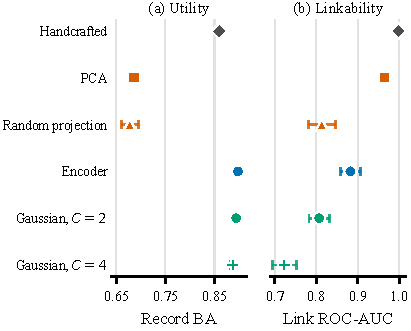
\includegraphics[width=\columnwidth]{main_utility_linkability_tradeoff.pdf}
\caption{Utility and linkability in the sample-matched comparison.}
\label{fig:main-tradeoff}
\end{figure}
\section{Discussion}
\label{sec:discussion}

Under the evaluated same-record protocol, feature extraction alone did not
eliminate linkability: handcrafted features preserved useful label information and
almost complete same-record separability. Among dimension-matched 8-D
representations, the encoder dominated PCA; random projection reduced
linkability further only with a large utility loss. Increasing the encoder to
64 dimensions left utility nearly unchanged but raised AUC from 0.882 to
0.941, so dimension contributed to, but did not explain, the trade-off.
Standardisation and selective-removal controls likewise reduced leakage only
slightly or at a material utility cost.

In the sample-matched comparison, the supervised bottleneck provided a
clearer change because it was learned for the intended utility task. The
dedicated operational reruns confirmed that the encoder and Gaussian
perturbation substantially reduced candidate retrieval. This is evidence that
task-oriented representation design can discard some record-specific
information under this protocol, not that supervised embeddings are
inherently private. The staged attack produced
small downstream changes under successful handcrafted-feature grouping: the
paired-bootstrap intervals excluded zero for sex balanced accuracy and
continuous-age MAE, but the effect sizes were modest and the binary age-group
interval crossed zero. Lower link precision prevented comparable
attacker-selected changes for the encoder conditions. Absolute performance
nevertheless remained above both the no-information and utility-only baselines
for handcrafted features. Gaussian perturbation approached the utility-only baseline,
especially for age-group classification. This distinction separates
background attribute predictability from representation-specific exposure and
from the incremental effect of attacker-selected linkage.

Direct reconstruction was independent of grouping. Its 128-component target
already imposed a substantial PRD floor, and both decoder families recovered
little from handcrafted features. Yet handcrafted features remained highly linkable: weak
inversion did not imply unlinkability. Neither oracle nor attacker-selected
means improved the linkage-conditioned attack; averaging instead removed
anchor-specific information. This finding is limited to feature-wise means and
does not exclude sequence-aware, generative, morphology-aligned, direct-waveform, or
auxiliary-data attacks.

Three limitations especially constrain generalisation. First, configuration
screens used the same source and were not nested within the final evaluation;
freezing settings prevents per-seed retuning but not selection optimism.
Second, three fixed seeds provide coarse between-run uncertainty, so the
standard deviations, $t$ intervals, and pooled bootstrap intervals are
descriptive and conditional. Third, clinical utility is restricted to binary
AF/AFL versus non-atrial classification using a record-derived label; it does
not demonstrate preservation of multiclass diagnosis, morphology, prognosis,
rare-rhythm detection, or other downstream tasks. In addition, the dataset has
one 10-s record per patient, the gallery is synthetic and closed set, and the
attribute attack is not external. Reconstruction is limited to one segment
position, 100-Hz targets, two decoder families, and feature-wise means. Fixed
budgets do not measure scaling, and Gaussian perturbation is not end-to-end
differential privacy.

\section{Conclusion}
\label{sec:conclusion}

Handcrafted ECG features preserved strong same-record linkability and
supported attribute inference above both baselines, although attacker-selected
linkage added little. A supervised bottleneck outperformed dimension-matched
PCA on utility and linkability; Gaussian perturbation further reduced pairwise
and gallery linkage while retaining useful performance on the single AF/AFL
classification task. The tested direct
reconstruction attacks were weak, and oracle or attacker-selected mean grouping
did not improve linkage-conditioned inversion. Thus, linkability, attribute
inference,
and reconstruction require separate evaluation rather than an irreversibility
claim. These results remain conditional on non-nested configuration selection,
three-seed uncertainty, the narrow utility task, the same-record protocol,
and the tested representation, aggregation, target, and attacker classes; they
do not establish
cross-session resistance, complete anonymisation, or end-to-end differential
privacy.

% Main-paper tables appear with their Results subsections; Figure~1 concludes Results.

\section*{Ethics Statement}
No new data were collected, and no participants were contacted. PhysioNet
reports institutional review-board approval at Shaoxing People's Hospital and
Ningbo First Hospital, waived consent, and public release after de-identification
\cite{Zheng2022PhysioNetECG}.

\section*{Data and Code Availability}
The source ECG recordings are publicly available from PhysioNet under the
Creative Commons Attribution 4.0 International license. Code, configurations,
and derived result tables will be released at
\url{https://github.com/tjpoa/ecg-privacy} before publication, with the final
manuscript archived as a tagged release.

% Extended tables are preserved in the source repository but excluded from the
% eight-page submission PDF. Set this switch to true only for an unconstrained
% archival build.
\newif\ifincludeappendices
\includeappendicesfalse
\ifincludeappendices
\appendices

\section{Configuration Selection and Fixed Model Settings}
\label{app:configuration}

Table~\ref{tab:configuration-evidence} records the development-stage checks
that motivated the fixed study configuration. The three blocks use different
development protocols and are therefore not direct performance comparisons
across blocks. The final article results come from the subsequent controlled
three-seed runs. Bold candidates were retained. BA denotes utility balanced
accuracy, and AUC denotes pairwise linkability ROC-AUC. The model-family block
is a single-split check, the dimension block averages two seeds, and the
Gaussian block averages three operational reruns.

\begin{table}[ht]
\centering
\scriptsize
\setlength{\tabcolsep}{2.4pt}
\caption{Development checks used to select the configuration.}
\label{tab:configuration-evidence}
\resizebox{\columnwidth}{!}{%
\begin{tabular}{llcc}
\toprule
Screen & Candidate & Utility BA & Link AUC \\
\midrule
Utility probe & \textbf{Logistic regression} & \textbf{0.8318} & -- \\
Utility probe & XGBoost & 0.7754 & -- \\
Link attacker & Logistic regression & -- & 0.9962 \\
Link attacker & \textbf{XGBoost} & -- & \textbf{0.9983} \\
\midrule
Bottleneck & \textbf{8-D} & \textbf{0.8705} & \textbf{0.8942} \\
Bottleneck & 16-D & 0.8688 & 0.9118 \\
Bottleneck & 32-D & 0.8727 & 0.9348 \\
\midrule
Gaussian & No perturbation & 0.8650 & 0.8823 \\
Gaussian & $m=0.0969,C=2$ & 0.8536 & 0.8602 \\
Gaussian & \textbf{$m=0.1938,C=2$} & \textbf{0.8335} & \textbf{0.8084} \\
Gaussian & \textbf{$m=0.1938,C=4$} & \textbf{0.8115} & \textbf{0.7228} \\
Gaussian & $m=0.4845,C=4$ & 0.7019 & 0.5346 \\
\bottomrule
\end{tabular}
}
\end{table}

The logistic-regression utility model is a fixed linear probe of accessible
task information. XGBoost is a fixed nonlinear attacker intended to avoid an
artificially weak linkability or attribute test. Ridge and MLP reconstruction
models bracket linear and nonlinear inversion. Table~\ref{tab:fixed-settings}
lists the settings needed to reproduce these capacities; iteration counts are
upper bounds or fixed budgets, not evidence of global optimisation.
Across the three seeds, early stopping terminated the handcrafted, encoder, and
Gaussian MLP decoders after 23--24, 19--24, and 16--19 iterations,
respectively.

\begin{table}[ht]
\centering
\scriptsize
\caption{Fixed analysis settings.}
\label{tab:fixed-settings}
\begin{tabular}{@{}p{0.25\columnwidth}p{0.68\columnwidth}@{}}
\toprule
Component & Fixed configuration \\
\midrule
Utility probe & Median imputation; standardisation; logistic regression with
$L_2$, $C=1$, \texttt{lbfgs}, balanced class weights, 2,000-iteration cap,
and random state 42. \\
Linear controls & Train-fitted PCA (no whitening) and Gaussian random
projection; 8-D main comparison, 64-D sensitivity, and split seed. \\
Encoder & Median imputation and standardisation; MLP hidden layers 128/8,
with the final hidden activation released; ReLU, Adam, $\alpha=10^{-4}$,
batch 1,024, learning rate $10^{-3}$, 25-iteration cap, early stopping,
10\% validation, patience 8, split seed, and at most 40,000 balanced segments. \\
Link attacker & Absolute representation differences; binary-logistic XGBoost,
200 trees, depth 4, learning rate 0.05, row/feature subsampling 0.8, log-loss,
random state 42; 2,000 pairs per class, minimum gap 4, and at most three
positive pairs per record. \\
Attribute models & Median imputation; XGBoost classifier/regressor with 200
trees, depth 4, learning rate 0.05, row/feature subsampling 0.8, histogram
trees, four threads, and split seed. Classifiers used binary logistic loss,
log-loss evaluation, and the training class ratio; age used squared error/RMSE. \\
Ridge decoder & Median imputation and standardisation of released inputs;
standardised target-PCA scores; $\alpha=1$, intercept fitted, automatic solver. \\
MLP decoder & Same input/target scaling; squared-error loss; hidden layers
256/128; ReLU, Adam, $\alpha=10^{-4}$, batch 256, learning rate $10^{-3}$,
100-iteration cap, early stopping, 10\% validation, patience 10, and split seed. \\
Target PCA & 128 components, randomized SVD, three power iterations, split
seed, and training waveforms only; direct reconstruction quantifies the target
compression floor. \\
Gaussian release & Standardised embeddings; $m=0.1938$;
$C\in\{2,4\}$ and $\sigma\in\{0.3876,0.7752\}$. No nominal
$\epsilon/\delta$ parametrisation or end-to-end DP claim. \\
Software & scikit-learn 1.7.2, XGBoost 3.2.0, NumPy 2.2.6, pandas 2.3.3,
and SciPy 1.15.3. \\
\bottomrule
\end{tabular}
\end{table}

\section{Representation-Dimension Sensitivity}
\label{app:dimension}

Table~\ref{tab:dimension-appendix} separates the effects of representation
family and output dimension under the same records, shared 40,000-segment
training subset, sampled pairs, and three seeds as Table~\ref{tab:main-summary}.
At eight dimensions, the encoder dominated PCA on both utility and linkability;
random projection achieved lower linkability only with a 0.221 absolute loss
in segment balanced accuracy relative to the encoder. Increasing encoder
dimension from 8 to 64 changed segment utility by only $-0.0010$ while raising
pairwise ROC-AUC by 0.0587. Thus, dimensionality contributes to leakage, but
does not by itself account for the encoder's utility--linkability profile.
Values are means plus or minus standard deviations over three matched seeds.
Handcrafted features provide the uncompressed reference.

\begin{table}[ht]
\centering
\scriptsize
\setlength{\tabcolsep}{2.5pt}
\caption{Representation-dimension sensitivity.}
\label{tab:dimension-appendix}
\resizebox{\columnwidth}{!}{%
\begin{tabular}{lccc}
\toprule
Representation & Segment BA & Record BA & Pairwise AUC \\
\midrule
Handcrafted, 208-D & $0.8318\mathbin{\pm}0.0017$ &
$0.8597\mathbin{\pm}0.0028$ & $0.9986\mathbin{\pm}0.0002$ \\
PCA, 8-D & $0.6765\mathbin{\pm}0.0064$ &
$0.6860\mathbin{\pm}0.0093$ & $0.9651\mathbin{\pm}0.0029$ \\
PCA, 64-D & $0.8037\mathbin{\pm}0.0008$ &
$0.8348\mathbin{\pm}0.0015$ & $0.9818\mathbin{\pm}0.0005$ \\
Random projection, 8-D & $0.6436\mathbin{\pm}0.0133$ &
$0.6773\mathbin{\pm}0.0172$ & $0.8137\mathbin{\pm}0.0326$ \\
Random projection, 64-D & $0.7881\mathbin{\pm}0.0022$ &
$0.8228\mathbin{\pm}0.0007$ & $0.9355\mathbin{\pm}0.0072$ \\
Supervised encoder, 8-D & $0.8647\mathbin{\pm}0.0027$ &
$0.8978\mathbin{\pm}0.0013$ & $0.8825\mathbin{\pm}0.0248$ \\
Supervised encoder, 64-D & $0.8637\mathbin{\pm}0.0016$ &
$0.9010\mathbin{\pm}0.0020$ & $0.9411\mathbin{\pm}0.0035$ \\
\bottomrule
\end{tabular}
}
\end{table}

\section{Additional Linkability Metrics}
\label{app:eer}

Table~\ref{tab:eer-appendix} reports threshold-based separation for the final
encoder family. Pairwise and operational EER agree closely within each
condition despite their different sampling protocols. The handcrafted operational
run did not retain EER output and is therefore not reconstructed post hoc.
Values are means plus or minus standard deviations over three dedicated seeds.
Higher EER indicates weaker separation; 0.5 is the no-separation reference.

\begin{table}[ht]
\centering
\scriptsize
\caption{Pairwise and operational equal error rates.}
\label{tab:eer-appendix}
\begin{tabular}{lcc}
\toprule
Representation & Pairwise EER & Operational EER \\
\midrule
Supervised encoder & $0.2058\mathbin{\pm}0.0214$ & $0.2071\mathbin{\pm}0.0132$ \\
Encoder + Gaussian, $C=2$ & $0.2698\mathbin{\pm}0.0115$ & $0.2680\mathbin{\pm}0.0148$ \\
Encoder + Gaussian, $C=4$ & $0.3375\mathbin{\pm}0.0165$ & $0.3332\mathbin{\pm}0.0134$ \\
\bottomrule
\end{tabular}
\end{table}

\section{Attribute-Inference Endpoints}
\label{app:attributes}

Tables~\ref{tab:attribute-ba} and \ref{tab:attribute-mae} provide all staged
attribute endpoints. S is one segment, O is the true same-record oracle
aggregate, L is the attacker-selected aggregate, and R aggregates random
different-record segments. Link-selection precision was 0.949, 0.325, and
0.174 for handcrafted, encoder, and Gaussian $C=2$ representations, respectively. The
no-information baselines predict the training majority class or median age;
the utility-label-only baselines receive only the binary clinical task label.
Because neither baseline aggregates released segments, only S is applicable.
Both tables average the three seeds.

\begin{table}[ht]
\centering
\scriptsize
\caption{Categorical attribute balanced accuracy.}
\label{tab:attribute-ba}
\begin{tabular}{llcccc}
\toprule
Representation & Endpoint & S & O & L & R \\
\midrule
No information & Sex & 0.500 & -- & -- & -- \\
No information & Age $\geq65$ & 0.500 & -- & -- & -- \\
Utility label & Sex & 0.515 & -- & -- & -- \\
Utility label & Age $\geq65$ & 0.656 & -- & -- & -- \\
\midrule
Handcrafted & Sex & 0.686 & 0.705 & 0.702 & 0.558 \\
Handcrafted & Age $\geq65$ & 0.707 & 0.725 & 0.721 & 0.584 \\
Encoder & Sex & 0.565 & 0.593 & 0.566 & 0.520 \\
Encoder & Age $\geq65$ & 0.688 & 0.713 & 0.682 & 0.572 \\
Gaussian $C=2$ & Sex & 0.536 & 0.560 & 0.528 & 0.522 \\
Gaussian $C=2$ & Age $\geq65$ & 0.665 & 0.702 & 0.659 & 0.568 \\
\bottomrule
\end{tabular}
\end{table}

\begin{table}[ht]
\centering
\scriptsize
\caption{Continuous-age mean absolute error.}
\label{tab:attribute-mae}
\begin{tabular}{lcccc}
\toprule
Representation & S & O & L & R \\
\midrule
No information & 15.145 & -- & -- & -- \\
Utility label & 13.825 & -- & -- & -- \\
\midrule
Handcrafted & 11.563 & 11.081 & 11.162 & 14.704 \\
Encoder & 12.655 & 11.771 & 12.665 & 15.413 \\
Gaussian $C=2$ & 13.303 & 12.256 & 13.405 & 15.346 \\
\bottomrule
\end{tabular}
\end{table}

\section{Per-Lead Reconstruction Detail}
\label{app:reconstruction}

Table~\ref{tab:reconstruction-complete} reports every global endpoint for both
decoder families; Table~\ref{tab:reconstruction-leads} then provides the
per-lead distribution for the strongest handcrafted-feature attack. Global
values are means plus or minus standard deviations over three seeds. Lead~II
lag $r$ uses the $\pm250$-ms search, and spectral $r$ uses log-magnitude
spectra. In the per-lead table, correlation is mean [IQR] and PRD is median
[IQR]. The table pools 7069 record--seed observations. Lead-specific PRD
excludes 0--225 near-zero targets for which the ratio is undefined.

\begin{table*}[ht]
\centering
\scriptsize
\setlength{\tabcolsep}{4pt}
\caption{Complete waveform-reconstruction results.}
\label{tab:reconstruction-complete}
\begin{tabular}{lcccccc}
\toprule
Input/decoder & PRD (\%) & SNR (dB) & Mean-lead $r$ & Lead II $r$ & Lead II lag $r$ & Spectral $r$ \\
\midrule
Train mean & $100.006\mathbin{\pm}0.002$ & $-0.0005\mathbin{\pm}0.0001$ & $0.0002\mathbin{\pm}0.0011$ & $-0.0001\mathbin{\pm}0.0015$ & $0.218\mathbin{\pm}0.004$ & $0.606\mathbin{\pm}0.010$ \\
Target PCA & $53.967\mathbin{\pm}0.147$ & $5.496\mathbin{\pm}0.022$ & $0.820\mathbin{\pm}0.002$ & $0.906\mathbin{\pm}0.0005$ & $0.919\mathbin{\pm}0.001$ & $0.872\mathbin{\pm}0.0001$ \\
Handcrafted/Ridge & $96.703\mathbin{\pm}0.027$ & $0.323\mathbin{\pm}0.003$ & $0.171\mathbin{\pm}0.002$ & $0.184\mathbin{\pm}0.003$ & $0.311\mathbin{\pm}0.003$ & $0.668\mathbin{\pm}0.001$ \\
Handcrafted/MLP & $96.493\mathbin{\pm}0.042$ & $0.343\mathbin{\pm}0.006$ & $0.167\mathbin{\pm}0.001$ & $0.179\mathbin{\pm}0.002$ & $0.317\mathbin{\pm}0.005$ & $0.660\mathbin{\pm}0.003$ \\
Encoder/Ridge & $99.726\mathbin{\pm}0.135$ & $0.028\mathbin{\pm}0.014$ & $0.052\mathbin{\pm}0.003$ & $0.058\mathbin{\pm}0.004$ & $0.206\mathbin{\pm}0.007$ & $0.574\mathbin{\pm}0.008$ \\
Encoder/MLP & $99.217\mathbin{\pm}0.313$ & $0.078\mathbin{\pm}0.031$ & $0.073\mathbin{\pm}0.008$ & $0.085\mathbin{\pm}0.003$ & $0.256\mathbin{\pm}0.009$ & $0.628\mathbin{\pm}0.011$ \\
Gaussian $C=2$/Ridge & $99.900\mathbin{\pm}0.030$ & $0.010\mathbin{\pm}0.003$ & $0.045\mathbin{\pm}0.003$ & $0.052\mathbin{\pm}0.004$ & $0.209\mathbin{\pm}0.005$ & $0.578\mathbin{\pm}0.005$ \\
Gaussian $C=2$/MLP & $99.734\mathbin{\pm}0.129$ & $0.026\mathbin{\pm}0.013$ & $0.050\mathbin{\pm}0.006$ & $0.059\mathbin{\pm}0.003$ & $0.237\mathbin{\pm}0.006$ & $0.626\mathbin{\pm}0.004$ \\
\bottomrule
\end{tabular}
\end{table*}

\begin{table}[ht]
\centering
\scriptsize
\setlength{\tabcolsep}{2.0pt}
\caption{Per-lead reconstruction results.}
\label{tab:reconstruction-leads}
\begin{tabular}{lccc}
\toprule
Lead & Target-PCA $r$ & Handcrafted $r$, mean [IQR] & Handcrafted PRD, med. [IQR] \\
\midrule
I   & 0.875 & 0.187 [0.038, 0.295] & 99.0 [96.1, 100.5] \\
II  & 0.906 & 0.179 [0.031, 0.284] & 99.2 [96.4, 100.5] \\
III & 0.684 & 0.151 [0.010, 0.249] & 99.5 [97.4, 100.6] \\
aVR & 0.923 & 0.183 [0.036, 0.289] & 99.1 [96.2, 100.5] \\
aVL & 0.696 & 0.166 [0.019, 0.275] & 99.3 [96.7, 100.6] \\
aVF & 0.819 & 0.169 [0.021, 0.274] & 99.3 [96.8, 100.6] \\
V1  & 0.781 & 0.157 [0.006, 0.253] & 99.4 [97.3, 100.7] \\
V2  & 0.797 & 0.175 [0.006, 0.302] & 99.2 [96.1, 100.6] \\
V3  & 0.813 & 0.173 [0.007, 0.288] & 99.3 [96.3, 100.7] \\
V4  & 0.834 & 0.155 [0.000, 0.250] & 99.5 [97.2, 100.6] \\
V5  & 0.855 & 0.150 [0.003, 0.241] & 99.5 [97.4, 100.7] \\
V6  & 0.856 & 0.162 [0.009, 0.265] & 99.4 [96.8, 100.6] \\
\bottomrule
\end{tabular}
\end{table}

\clearpage
\fi
\bibliographystyle{IEEEtran}
\bibliography{overleaf_jbhi_submission/references}

\end{document}
